\documentclass[12pt]{article}
\usepackage{caption}
\usepackage{subcaption}


% Language setting
% Replace `english' with e.g. `spanish' to change the document language
\usepackage[english]{babel}

% Set page size and margins
% Replace `letterpaper' with `a4paper' for UK/EU standard size
\usepackage[letterpaper,top=2cm,bottom=2cm,left=2cm,right=2cm,marginparwidth=2cm]{geometry}

\usepackage{listings}

% Useful packages
\usepackage{amsmath}
\usepackage{graphicx}
\usepackage[colorlinks=true, allcolors=blue]{hyperref}

\title{Polytechnique Montreal \\
LOG8415: Lab 2\\
Mapreduce with Hadoop on AWS}

\author{Line Ghanem - 1728134\\Zineddine Aliche - 1949905\\
Mohammed Ramzi Bouthiba - 2065386\\Axelle Pagnier - 2164162}

\begin{document}
\maketitle

\begin{abstract}
In this assignment, we use an EC2 instance (M4.large type and under Linux Ubuntu operating system) of AWS to experiment with the MapReduce paradigm using two open source distributed computing frameworks: Hadoop and Spark. The assignment is composed of three parts, the first is for setting up the environments of Hadoop and Spark, the second is for the application of a text wordcount with Hadoop, spark and Linux, the last part concerns the application of experiments of the first two parts on a real problem which is the social network friendship recommendation.All the assignment is done in standalone mode.
\end{abstract}

\section{Setting Up the Environment}

In this section we are going to discuss the steps that lead to setting up an M4.large Linux Ubuntu EC2 instance on AWS and installing Hadoop and Apache Spark on the instance so that it is ready to run our experiments automatically.\newline

\noindent The first step is to setup an M4.large. To do that, we wrote a python script that retrieves the default VPC id and the default subnet id of that VPC. Then, create a security group  which contains a set of rules that filter incoming and outgoing traffic. We allowed HTTP and SSH connections from everywhere (0.0.0.0/0). After that we proceed to the creation of the M4.large instance in the us-east-1 region and associate it the retrieved VPC and subnet and the newly created security group. \newline

\noindent The second step is to prepare the environment of that EC2 instance such that it can run Hadoop and Apache Spark jobs. After creating the instance, we sent multiple bash files to that instance via the scp1 protocol. Those bash files are used to configure Hadoop and Spark to work properly. After sending those bash scripts to the instance, we used a python script to connect to the instance over SSH and download Java 11, Hadoop 3.3.1 and Spark 3.3.1 and put them in the appropriate directories, then launch the configuration bash files to set up Hadoop ans Spark properly.\newline

\noindent Among the files that we sent, we included bash script and Java MapReduce programs to run the Hadoop jobs and a python script to be used by pyspark to run the Spark job. we also sent bash script to launch the experiments that we are going to discuss in the next section.



\section{Experiments with WordCount}
\subsection{Hadoop vs. Linux}
In this part we compare the performance of hadoop and linux on a wordcount task, the performance measure is the real execution time to perform this task. For this purpose we used the contents of Ulysses as an input text file.The results are shown in figure 1.\newline
\begin{figure}[h]
    
     \begin{subfigure}[b]{0.41\textwidth}
         
         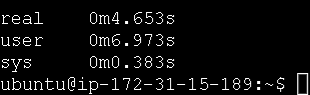
\includegraphics[width=\textwidth]{Hadoop_wordcount_Ulysses.png}
         
     \end{subfigure}
     \hfill
     \begin{subfigure}[b]{0.41\textwidth}
         
         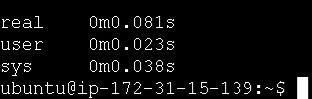
\includegraphics[width=\textwidth]{Linux_wordcount_Ulysses.png}
         
     \end{subfigure}
     \hfill
        \centering
        \caption{Comparison of Hadoop and Linux on the wordcount of the contents of Ulysses. On the right Linux and on the left Hadoop}
        \label{fig:three graphs}
\end{figure}

\noindent The results obtained show that Linux perform this task 58 times faster compared to Hadoop.

\subsection{Hadoop vs. Spark}
For this part, we compare the execution time of Hadoop and Spark on a dataset that contains 9 text files. We used Python (PySpark) as the programming language for Spark and Java for Hadoop. We ran the program 3 times for each text file and took the average time.Spark runtime result is multiplied by \textbf{10}(in order to show it well on the graph). It should be noted that for spark we give the data file directly without going through HDFS. The results are shown in Figure 2.

\begin{figure}[h]
  \centering
  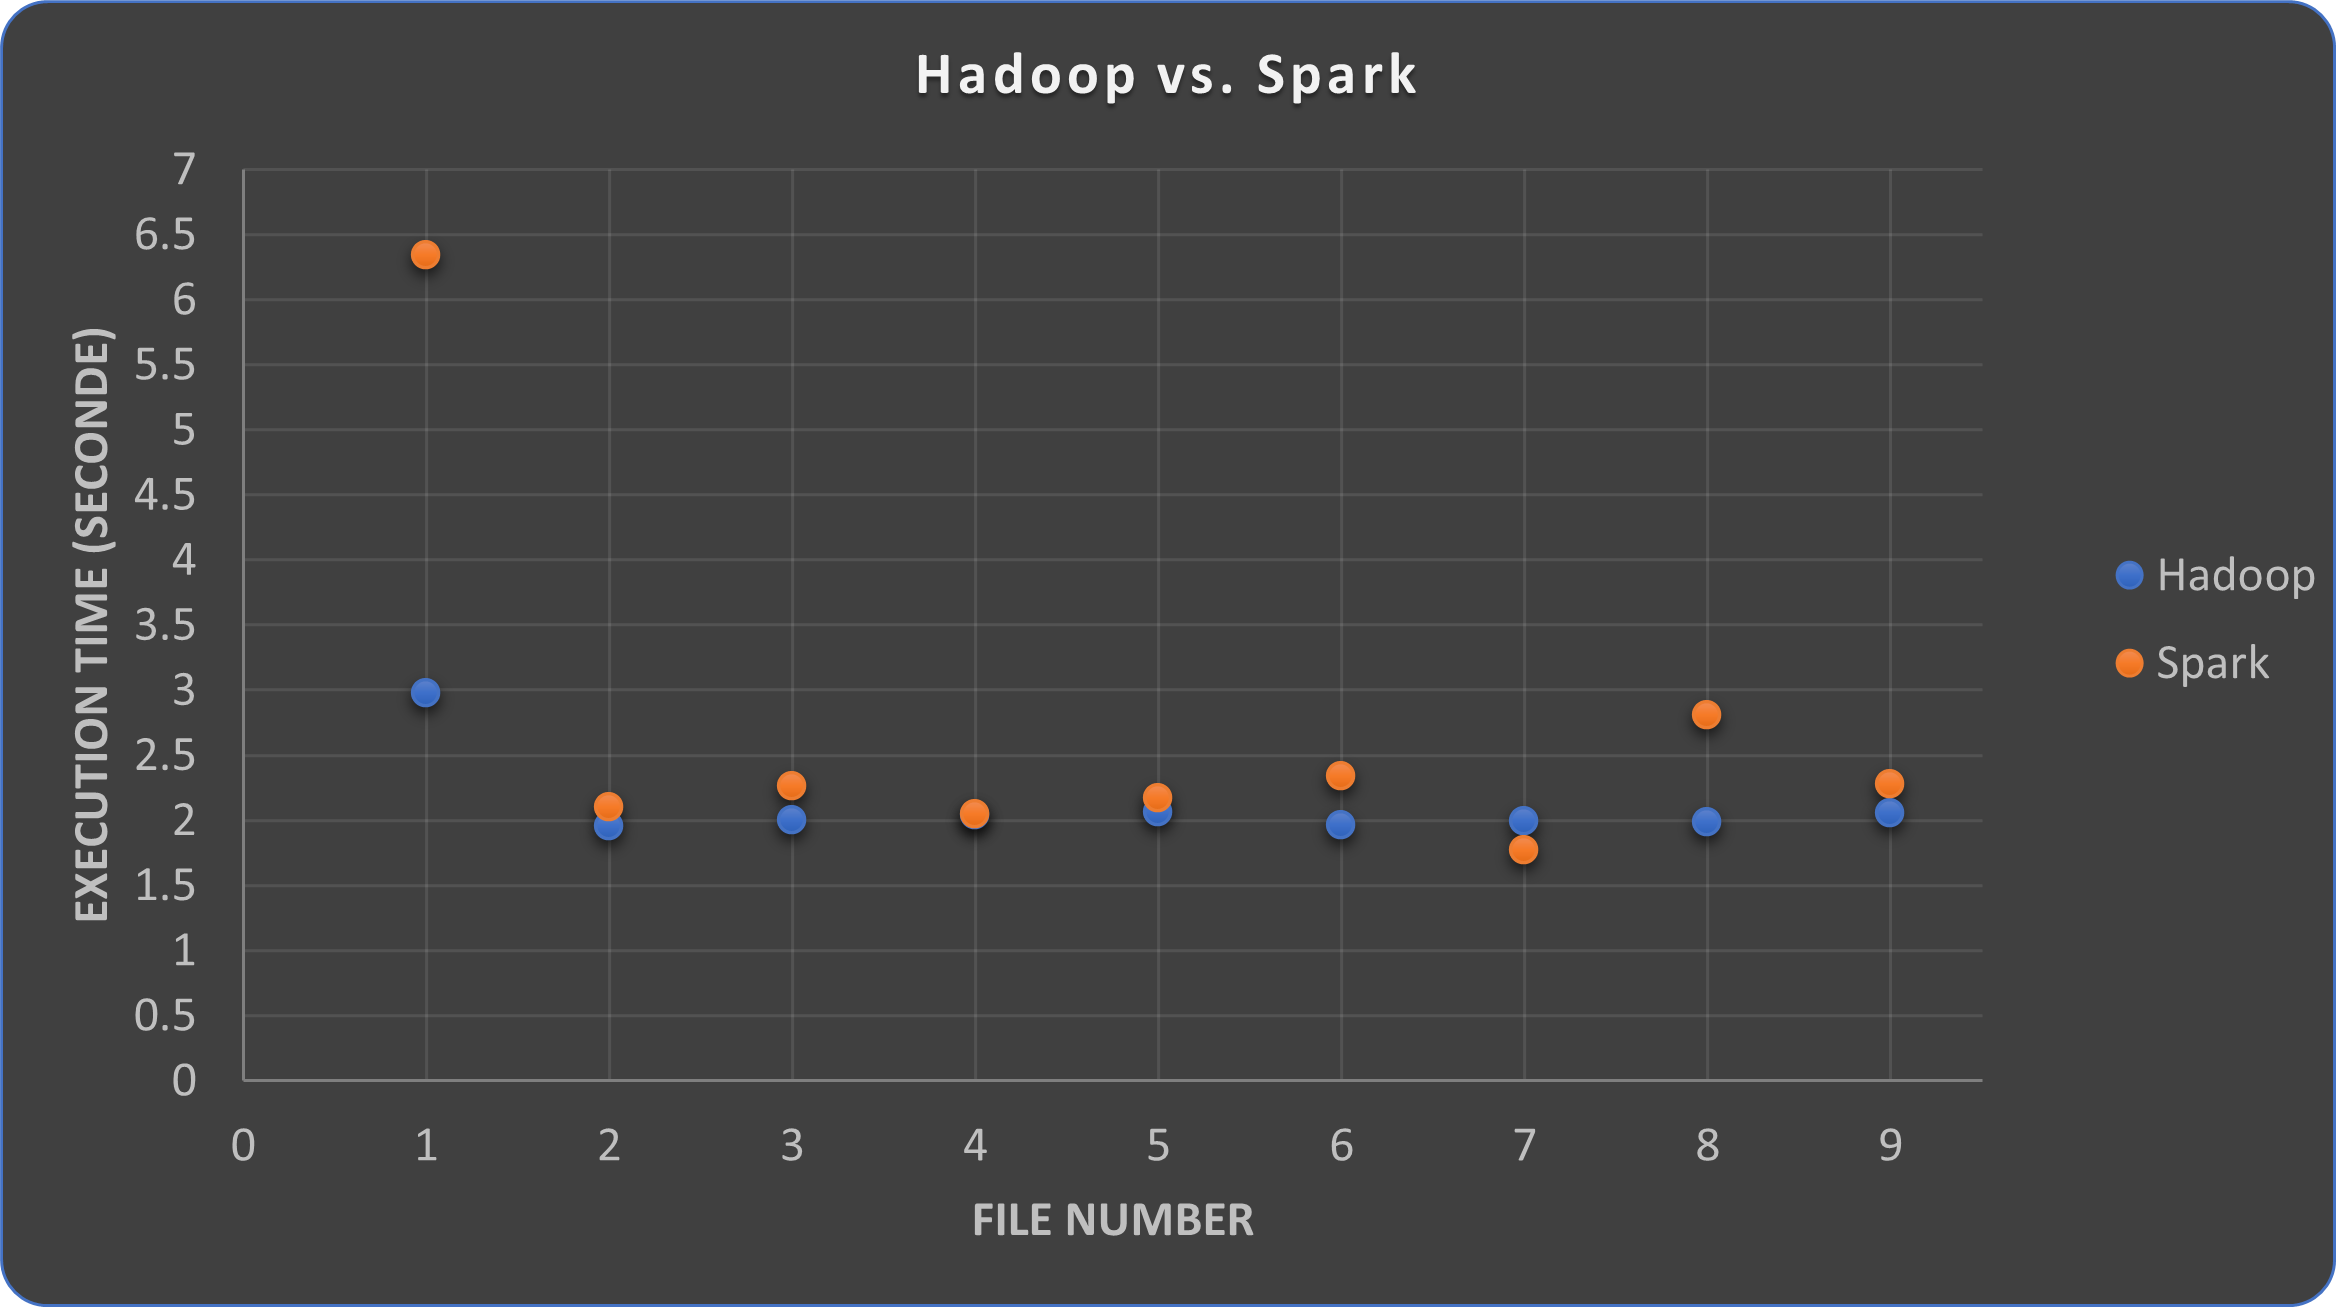
\includegraphics[scale=0.65]{Hadoop vs spark.png}
  \caption{Execution time of Hadoop (1xT) and Spark (10xT).}
  \label{fig:hadoop vs spark}
\end{figure}
It can be seen from figure 2 that the execution time is greater for Hadoop compared to Spark .\\
The main reason for this difference is that Spark processes data in-memory while Hadoop Mapreduce returns to disk after each step of map or reduce.Through this experience it was confirmed that Spark performs well as Hadoop.
\section{Social network friendship recommendation}
In this section we will describe a solution to the following problem:
give 10 friends recommendation to each user based on their mutual friends.
For each user we will return the 10 recommendations with who the user has the biggest number of mutual friends. Since we are using Hadoop MapReduce to solve the problem we have divided our implementation in two phases Map and Reduce using the java \textbf{org.apache.hadoop} packages. An important concept in Hadoop MapReduce is the context. The context allow the mapper and the reducer to communicate with the rest of the system and most importantly it stores values across map and reduce jobs. 


The Map section will first map each friend to his first degree friends as follows: \textbf{(UserKey, (Friend, -1))}.
Then, for each friend in the friend list of the user we will create a second degree relationship as follows: \textbf{(Friend1, (Friend2, 1))} and \textbf{(Friend2, (Friend1, 1))}. Note a relationship with 1 means they are second degree friends and a relationship with -1 means they are first degree friends. Each of the entries created in the map phase are added to the context (Figure \ref{fig:map}).
\begin{figure}[h]
  \centering
  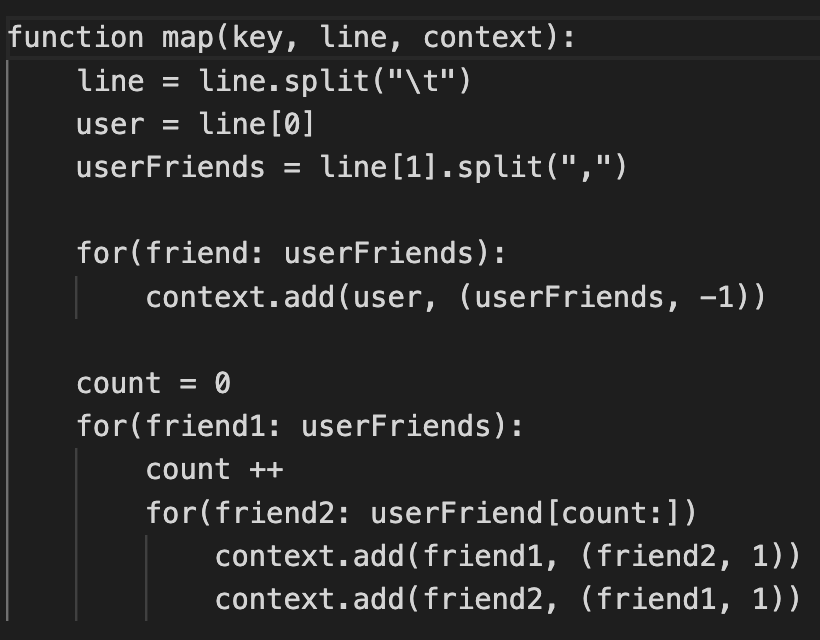
\includegraphics[scale=0.65]{map.png}
  \caption{Pseudo code of the mapper function.}
  \label{fig:map}
\end{figure}

In the reduce phase, for each UserKey, we count the number of mutual friends that each user has with the same second degree friend. To do this we will use the context entries created in the map phase. For example, given user A and B if the relationship (A, (D, 1)) is counted 2 times the number of mutual friends between A and D is 2. However, if the following entry existed: (A, (B,-1)); A and B are first degree friends and the count is set to -1 since first degree friends will not be recommended to each other (Figure \ref{fig:reduce}).

\begin{figure}[h]
  \centering
  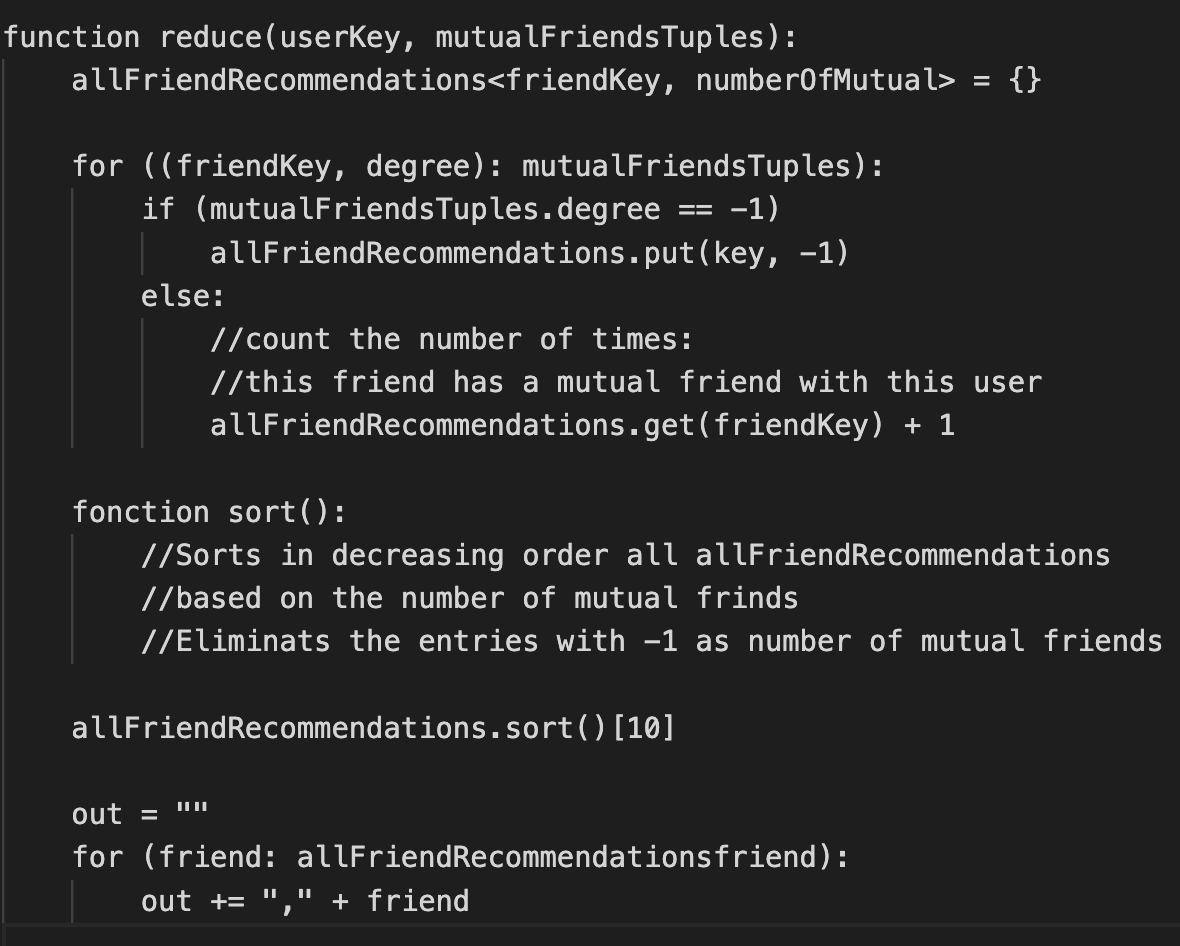
\includegraphics[scale=0.65]{reduce.png}
  \caption{Pseudo code of the reducer function.}
  \label{fig:reduce}
\end{figure}

A short example of the logic is seen in Figure \ref{fig:mapreduce}.

\begin{figure}[h]
  \centering
  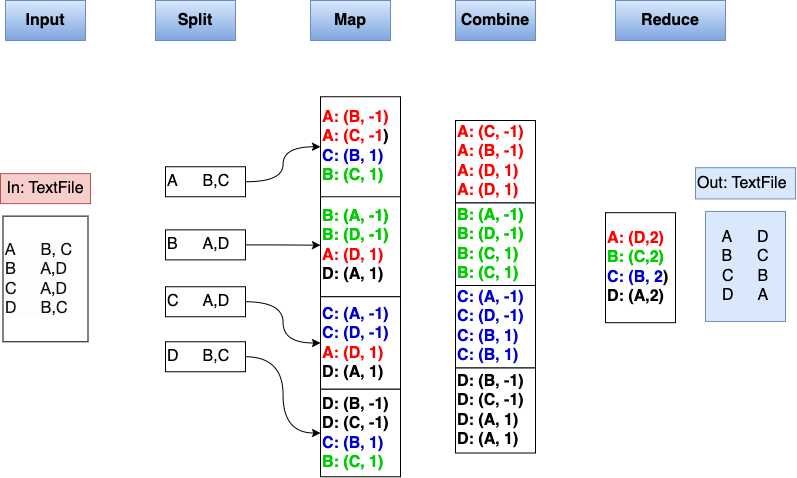
\includegraphics[width=\linewidth]{mapreduce.png}
  \caption{Simplified example of the MapReduce solution for the networking problem.}
  \label{fig:mapreduce}
\end{figure}

\paragraph{Results of networking problem:} (Table below)

\begin{center}
\begin{tabular}{c|c}[h]
  User & Top 10 recommended friends\\
  \hline\hline
  924  &   439,2409,6995,11860,15416,43748,45881\\
  8941  &  8943,8944,8940\\
  8942   & 8939,8940,8943,8944\\
  9019  &  9022,317,9023\\
  9020   & 9021,9016,9017,9022,317,9023\\
  9021   & 9020,9016,9017,9022,317,9023\\
  9022   & 9019,9020,9021,317,9016,9017,9023\\
  9990   & 13134,13478,13877,34299,34485,34642,37941\\
  9992  &  9987,9989,35667,9991\\
  9993  &  9991,13134,13478,13877,34299,34485,34642,37941\\  
\end{tabular}
\end{center}
\section{Conclusion}
In this lab, we used Hadoop and Spark to conduct wordcount experiments and the social network friendship recommendation problem. A first experiment was made to compare Hadoop and Linux in a wordcount task, the results obtained show that Linux is very fast compared to Hadoop because Hadoop stores data on multiple sources (HDFS) and processes it in batches via MapReduce.
A second experiment was conducted to compare the performance of Hadoop and Spark and the result obtained illustrates that Spark is faster than Hadoop and this because Spark RAM instead of reading and writing intermediate data to disks.
A last experiment is made on a real problem of social network friendship recommendation in order to make a friend suggestion for a user based on the number of mutual friends in common with that user.



 


\end{document}